\section{Zielsetzung}
\label{sec:Zielsetzung}
In Versuch 500 wird die Auslösung von Elektronen aus einer Metalloberfläche durch Bestrahlung mit Photonen untersucht.
Dabei wird die Abhängigkeit der Energie der ausgelösten Elektronen von der Wellenlänge des einfallenden Lichts beobachtet.

\section{Theorie}
\label{sec:Theorie}
Licht lässt sich klassisch nicht eindeutig dem Korpuskel- oder dem Wellenmodell zuordnen. So erfordert der lichtelektrische Effekt und der Compton-Effekt eine
Beschreibung als Teilchen. Jedoch lassen sich Phänomene wie die Interferenz oder die Beugung nur mit der Wellentheorie erklären.
Die Quantenmechanik vereint allerdings beide Modelle als Grenzfälle. Lässt sich über eine große Anzahl von Photonen mitteln, so wird die Beschreibung als Welle verwendet.
Bei Wechselwirkungen des Lichts mit Materie dient das Korpuskelmodell als Beschreibung.
\\
\\
Da beim Photoeffekt eine Wechselwirkung stattfindet, wird die Beschreibung des Photons als Teilchen benötigt. Um den Photoeffekt zu realisieren wird eine Metallplatte (Photokathode)
mit monochromatischem Licht bestrahlt. Gegenüber befindet sich eine Auffängerelektrode, die ein positives Potential im Bezug zur Photokathode aufweist.
Die beiden Platten sind über ein Amperemeter verbunden, wodurch der abfließende Strom gemessen wird. Der Strom entsteht dadurch, dass die Elektronen durch die Potentialdifferenz
zur Auffängerelektrode hin beschleunigt werden. Der schematische Aufbau einer solchen Anordnung ist in \autoref{fig:schema} skizziert.
\begin{figure}[H]
    \centering
    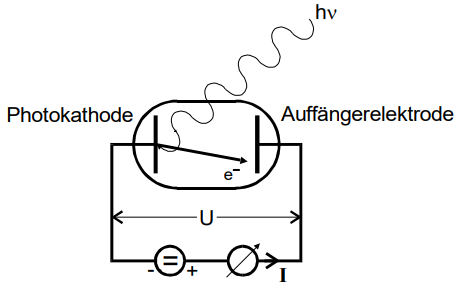
\includegraphics[width=0.5\textwidth]{img/schema.png}
    \caption{Schematischer Aufbau zur Herbeiführung des Photoeffekts \cite{V500}.}
    \label{fig:schema}
\end{figure}

Beim lichtelektrischen Effekt gilt, dass sich die Anzahl der herausgelösten Elektronen proportional zur Lichtintensität verhält und die maximale kinetische Energie der Elektronen
proportional zur Lichtfrequent und unabhängig von der Lichtintensität ist. 
Desweiteren existiert eine Grenzfrequenz unter der der Effekt nicht auftritt.
Klassisch ist dieses Verhalten nicht mit dem Wellenmodell vereinbar. Wird nun jedoch angenommen, dass sich die Energie in einem infinitesimalen Teilchen konzentriert, ist das
genannte Verhalten erklärbar. Diese infinitesimalen Teilchen werden Photonen genannt. Ihre Energie berechnet sich mit
\begin{equation*}
    E_{Ph} = h \cdot f.
\end{equation*}
Dabei ist $E_Ph$ die Photonenenergie, $h$ das Plank'sche Wirkungsquantum und $f$ die Frequenz des Lichtes.
Beim Photoeffekt wird diese Energie beim Auftreffen auf das Kathodenmaterial auf die Elektronen übertragen. Ist die Energie des Photons groß genug, um die 
Austrittsarbeit $A_k$ zu leisten, verlässt das Elektron die Platte. Die Austrittsarbeit $A_k$ ist dabei materialspezifisch. Die überschüssige $E_{Ph}$ erhält dann das 
herausgelöste Elektron als kinetische Energie $E_{kin}$. Folglich gilt
\begin{equation*}
    hf = E_{kin} + A_k.
\end{equation*}
Daraus lässt sich auch direkt ein Schluss auf die Grenzfrequenz ziehen. Gilt nämlich
\begin{equation*}
    f < \frac{A_k}{h}
\end{equation*}
so kann der Photoeffekt nicht mehr auftreten.
